\documentclass[12pt]{article}
\usepackage[spanish]{babel}
\usepackage{geometry}
\geometry{a4paper, margin=1in}
\usepackage{graphicx}
\usepackage{xcolor}
\usepackage{titlesec}
\usepackage{parskip}
\usepackage{multicol}
\usepackage{cite}

\definecolor{highlight}{RGB}{255, 255, 0}

\titleformat{\section}{\normalfont\Large\bfseries}{\thesection}{1em}{}
\titleformat{\subsection}{\normalfont\large\bfseries}{\thesubsection}{1em}{}

\begin{document}

% Logos
\begin{minipage}{0.45\textwidth}
    
\includegraphics[width=0.4\textwidth]{inFiles/Figures/epnLogo.jpg}
\end{minipage}
\hfill
\begin{minipage}{0.45\textwidth}
    \raggedleft
    
\includegraphics[width=0.4\textwidth]{inFiles/Figures/FIS_logo.jpg}
\end{minipage}

\vspace{0.5cm}

% Títulos principales
\begin{center}
    \textbf{ESCUELA POLITÉCNICA NACIONAL}\\[0.2cm]
    \textbf{FACULTAD DE INGENIERÍA DE SISTEMAS}\\[0.2cm]
    \textbf{INGENIERÍA COMPUTACION}
\end{center}

\vspace{0.5cm}
\hrule
\vspace{0.5cm}

% Datos principales
\noindent\textbf{PERÍODO ACADÉMICO:} 2025-A\\[0.2cm]
\noindent\textbf{ASIGNATURA:} ICCD412 Métodos Numéricos \hfill \textbf{GRUPO:} GR2CC\\[0.2cm]
\noindent\textbf{TIPO DE INSTRUMENTO:} DEBER\\[0.2cm]
\noindent\textbf{FECHA DE ENTREGA LÍMITE:} {04/05/2025}\\[0.2cm]
\noindent\textbf{ALUMNO:} Contreras Carrión Anthony Alexander

\vspace{0.5cm}
\hrule
\vspace{1cm}


% Secciones
\section*{TEMA}
Tipo de Errores


\section*{OBJETIVOS}
\begin{itemize}
    \item Investigar los límites de Python en el manejo de grandes volúmenes de datos, analizando fallos por desbordamiento o tamaño excesivo.
\end{itemize}


\section*{DESARROLLO}

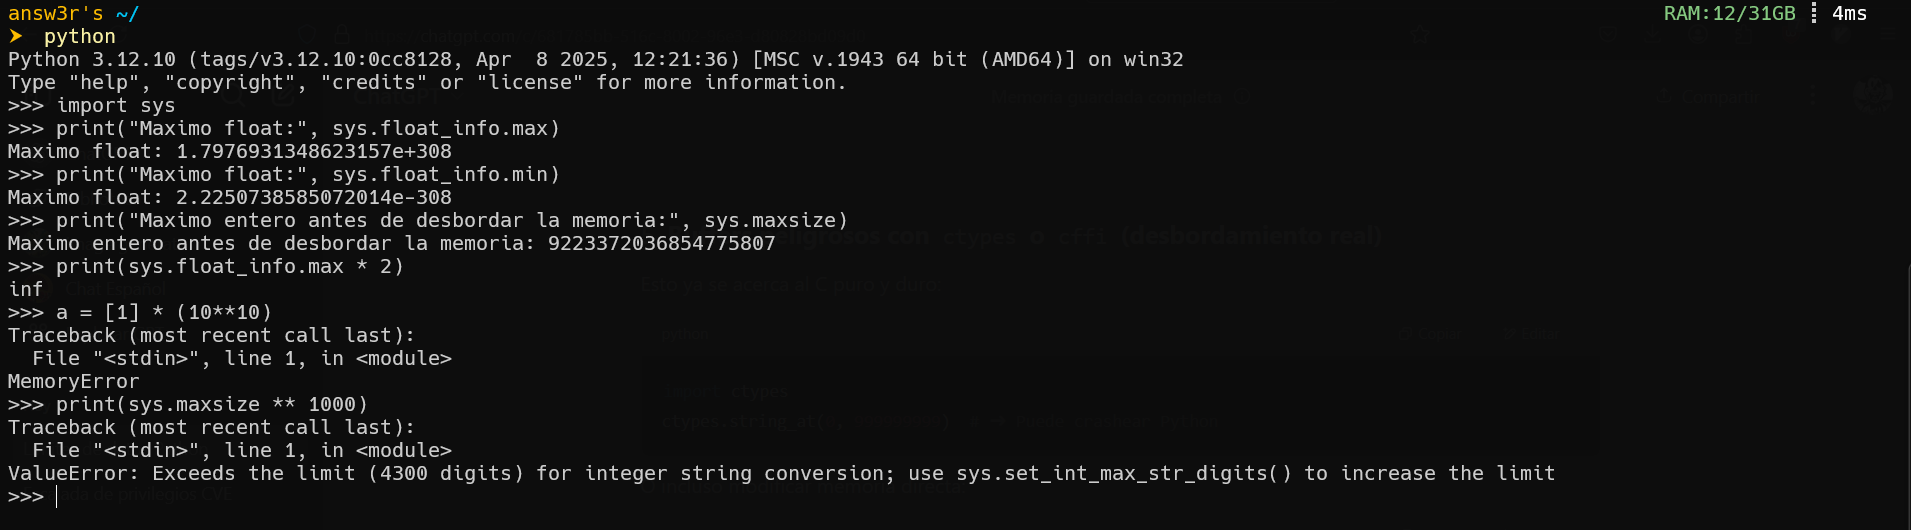
\includegraphics[width=0.98\textwidth]{inFiles/Figures/python.png}
\vspace{0.5cm}

\section*{CONCLUSIONES}

Se puede evidenciar que, cuando trabajamos con números extremadamente grandes, Python devuelve inf
 (infinito) como una forma de representar un valor que excede el límite 
numérico manejable por el tipo de dato flotante. Además, al realizar 
multiplicaciones de gran magnitud, Python impone ciertas restricciones 
para evitar un consumo excesivo de recursos del sistema, lo cual también
 sirve como una medida de protección contra ataques de denegación de 
servicio (DoS).

\end{document}
